\section{Pregunta N$^{\circ}$13\qquad Leon Alonzo Terrones Caccha}

\begin{frame}
    \begin{enumerate}\setcounter{enumi}{12}
        \item

              Obtenga el polinomio trigonométrico de mínimos
              cuadrados continuos $S_{3}\left(x\right)$ para
              \begin{math}
                  f\left(x\right)=
                  x^{2}\sin
                  \left(x^{2}\right)
              \end{math}
              en
              \begin{math}
                  \left[-\pi,\pi\right]
              \end{math}.
    \end{enumerate}

    \begin{solution}
        Sea el polinomio trigonométrico de grado $3$
        \begin{equation*}
            S_{3}\left(x\right)=
            \dfrac{a_{0}}{2}+
            a_{3}\cos\left(3x\right)+
            \sum_{k=1}^{2}
            \left[
                a_{k}\cos\left(kx\right)+
                b_{k}\operatorname{sen}\left(kx\right)
                \right],
        \end{equation*}
        donde
        \begin{align*}
            a_{k} & =
            \dfrac{1}{\pi}
            \int\limits_{-\pi}^{\pi}
            f\left(x\right)\cos\left(kx\right),\quad
            \forall k\in\left\{0,\dotsc,n\right\} \\
            b_{k} & =
            \dfrac{1}{\pi}
            \int\limits_{-\pi}^{\pi}
            f\left(x\right)\operatorname{sen}\left(kx\right),\quad
            \forall k\in\left\{1,\dotsc,n-1\right\}.
        \end{align*}
    \end{solution}
\end{frame}

\begin{frame}{Implementación}
    \begin{figure}
        \centering
        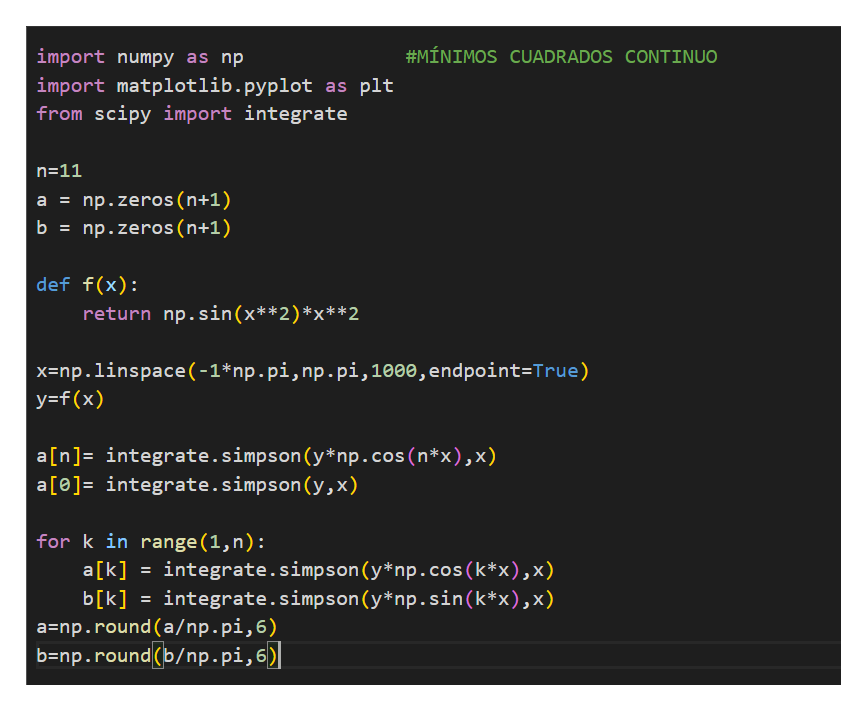
\includegraphics[width=.7\paperwidth]{p13-code1.png}
    \end{figure}
\end{frame}

\begin{frame}{Implementación}
    \begin{figure}
        \centering
        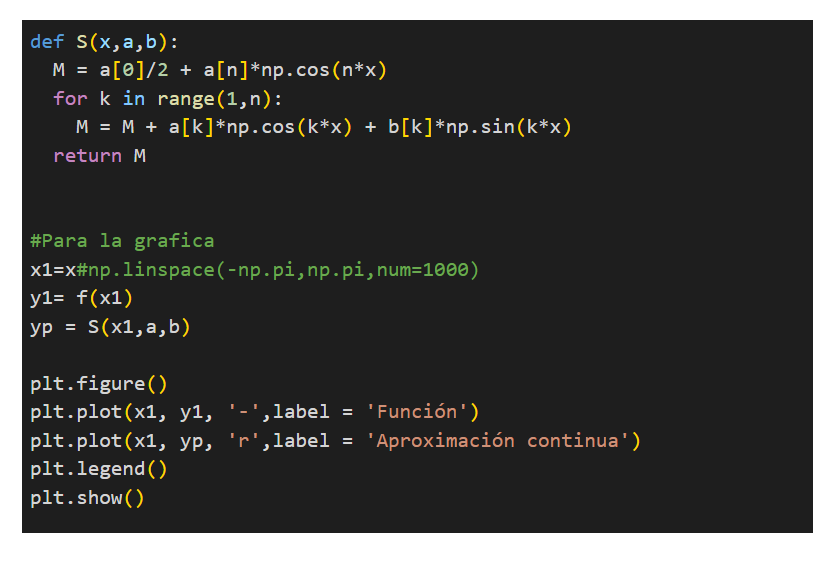
\includegraphics[width=.82\paperwidth]{p13-code2.png}
    \end{figure}
\end{frame}

\begin{frame}{Resultados}
    \begin{figure}
        \centering
        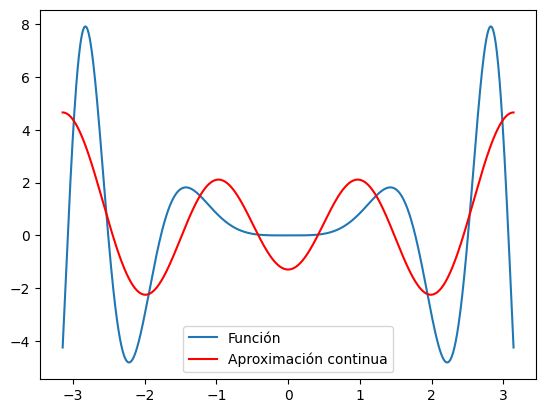
\includegraphics[width=.75\paperwidth]{p13-Aprox-continua.png}
        \caption{Para $n=3$}
    \end{figure}
\end{frame}

\begin{frame}{Resultados}
    \begin{figure}
        \centering
        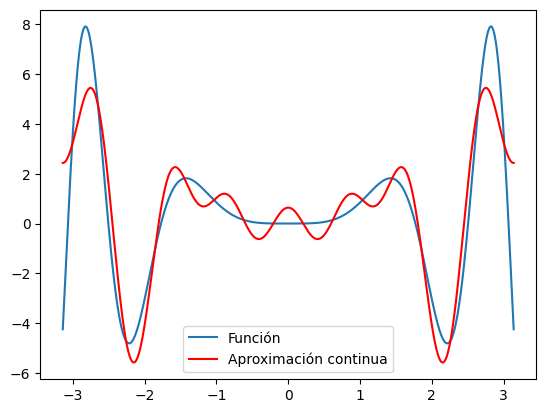
\includegraphics[width=.75\paperwidth]{p13-A-continua.png}
        \caption{Para $n=7$}
    \end{figure}
\end{frame}

\begin{frame}{Resultados}
    \begin{figure}
        \centering
        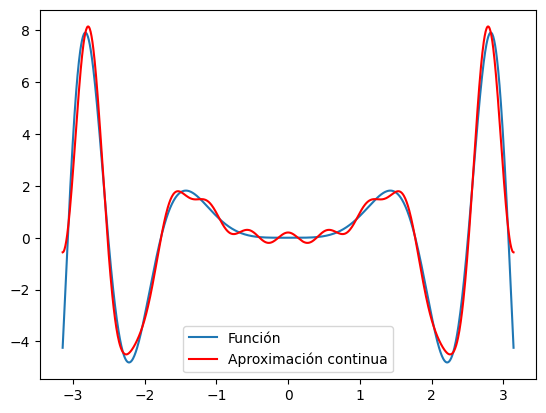
\includegraphics[width=.75\paperwidth]{p13-A-cont3.png}
        \caption{Para $n=11$}
    \end{figure}
\end{frame}